%! Author = Saeid Yazdani
%! Date = 1/9/2024


\section{Test Equipment Role in Electronics Industry}
\label{sec:importance-ate-in-semiconducor}

Testing components is time- and cost-intensive, specially when evaluating 
mass-produced consumer devices. \acp{ATE} provide a structured environment 
to perform functional, parametric, and system-level tests efficiently during 
the fabrication and verification phases. As illustrated in 
\autoref{fig:semiconductor-ecosystem}, \acp{ATE} play a central role in the 
semiconductor ecosystem by supporting the engineering, design, and testing 
processes to ensure that only functional and specification-compliant devices 
are released to the market.

\begin{figure}[htbp]
    \centering
    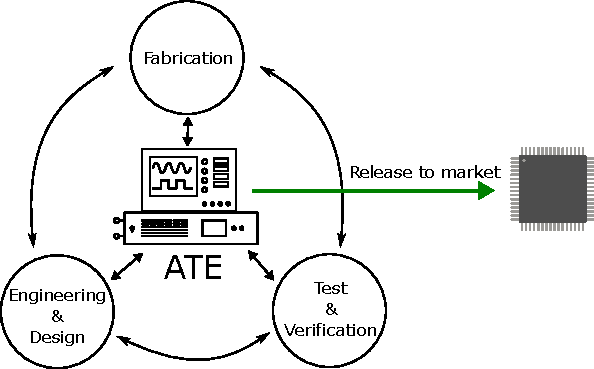
\includegraphics[width=\linewidth,height=0.62\textheight,keepaspectratio]{figures/semiconductor_ecosystem}
    \caption[ATE Semiconductor ecosystem]{\ac{ATE} systems play a central role in the 
    semiconductor ecosystem by supporting fabrication, engineering, and testing 
    processes to ensure that devices meet functional and specification requirements 
    before release to the market.}
    \label{fig:semiconductor-ecosystem}
\end{figure}

\subsection{Challenges with test equipment}
\label{subsec:challenges-test-equipment}

The rate of progress in semiconductor fabrication techniques is outpacing the
progress in the design of hardware testers, especially on the power supply
circuits and their associated control loops responsible for generating
test signals and
powering up \acp{DUT} \autocite{paper:vlsi-highcurrent-test,article:suri}.

In recent years, the fabrication process technology of semiconductors has
miniaturized, and as a direct result, supply voltages became significantly
lower compared to former fabrication processes.
Meanwhile, the electrical current consumption of these semiconductors has
increased due to the vast number of transistors packed in
a small area \autocite{Ishida}.
This has increased the power supply noise and power integrity issues of
\acp{DUT}, and there maybe a gap between test and
operational conditions which has become a serious concern \autocite{Arabi}.

\ac{DUT} power supplies of \ac{ATE} systems are responsible for generating
test waveforms in a wide range of voltage and current levels and timing
dynamics.
A general-purpose \ac{ATE} should be able to generate low to high levels of
voltage and current while maintaining signal timings close to
test requirements for any given \ac{DUT}, as the test signals should not exhibit
unwanted behaviors such as \emph{overshoot}, \emph{undershoot} and
\emph{voltage drop} that may invalidate test runs or lead to false-positive
results.

A modern \ac{CPU} in an idle state would require a steady supply of \SI{0.8}{\volt} and 
\SI{0.1}{\ampere}, but at the instance of a clock transition in load operation, the \ac{CPU} 
can demand \SI{1.3}{\volt} and \SI{100}{\ampere} within tens of nanoseconds
\autocite{792807}. As processor speeds increase and systems frequently transition between 
sleep and active modes, managing such large, rapid load changes has become increasingly 
important.

Power delivery to the \ac{DUT} can be customized for any particular \ac{DUT},
and socket placement and load board routing should be optimized when it comes to
parasitic \ac{RLC} components.

Test and characterization of passive and active components, such as resistors
and diodes are another application for ATE SMU systems.
\acp{SMU} are used in production facilities and we test each and every component
to check functional correctness prior to releasing to the market.
Examples are curve tracing of diodes, resistor correction, and drain-source
check on \acs{MOSFET}s. In this application, the speed of the tester is essential
to keep throughput as high as possible.

\begin{figure}[h]
    \centering
    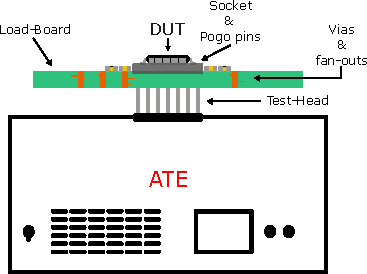
\includegraphics[scale=1.32]
    {figures/ate-to-dut-wiring}
    \caption[ATE to DUT wiring]{A Typical wiring scheme between ATE power supply
    and DUT. Each object in the path contributes to the overall
    performance and response of the power supply due to introduced parasitics.}
    \label{fig:ate-to-dut}
\end{figure}


\section{What needs to be done}
\label{subsec:what-needs-to-be-done}

What can be
improved in \ac{ATE} systems in response to challenging \ac{DUT} power
requirements is the control loop of power supplies.
Power stage components such as power transistors, high-bandwidth amplifiers with
suitable properties like slew-rate and gain response already exist in the
market.
The control loop design can be further enhanced to respond faster, cleaner,
and safer.

Therefore, there is a demand for new and improved control methods,
in the power supply market in general and ATE market in particular;
that can benefit from digital circuitry and software control to eliminate the
shortcomings of purely analog-based power supplies.
Exploring new solutions for power supplies and control loops, as explained later
in this text, can also lead to reduced component count, reduced physical
footprint, increased reliability, and flexibility.
